\documentclass{beamer}
\usepackage[utf8]{inputenc}
\usepackage[T1]{fontenc}

\setbeamerfont{title}{size=\LARGE}

\title{Linux a jeho historie}
\author{Eliška Jégrová}
\date{13.03.2024}

\begin{document}
	
	\frame{\titlepage}


% Slide 1: Definice Linuxu
\begin{frame}{Definice Linuxu}
	\begin{block}{Co je to ten „Linux“?}
		    \begin{columns}
			\begin{column}{0.7\textwidth}
				% Text on the left side
				\begin{itemize}
					\item Linux je název jádra (kernelu) operačního systému.
					\item Zajišťuje komunikaci s hardwarem a umožňuje běh ostatních programů.
					\item Systém se skládá z různých komponent zajišťujících spouštění programů, grafické rozhraní, síťovou konektivitu a další.
				\end{itemize}
			\end{column}
			\begin{column}{0.3\textwidth}
				% Image on the right side
				\includegraphics[height=3cm]{tux.png}
			\end{column}
		\end{columns}
	\end{block}

	\begin{block}{Otevřený Zdrojový Kód (Open Source)}
		\begin{itemize}
			\item Software s otevřeným zdrojovým kódem, umožňující úpravy a sdílení.
		\end{itemize}
	\end{block}
\end{frame}


% Slide 2: Varianty Linuxu
\begin{frame}{}
	\begin{block}{Komponenty v Operačních Systémech}
		\begin{itemize}
			\item \textbf{Jádro systému} – Linux, FreeBSD, OpenBSD, …
			\item \textbf{Shell} – Bash, zsh, csh, Fish, Xonsh, sh, …
			\item \textbf{Základní nástroje} – GNU coreutils, BusyBox, …
			\item \textbf{Balíčkovací systém} – DNF, APT, pacman, …
			\item \textbf{Správce služeb} – systemd, upstart. openrc, init, …
			\item \textbf{Textový editor} – Gedit, Kate, vim, Emacs, Atom, nano, …
   		    \item \textbf{Grafické prostředí} – GNOME, KDE Plasma, XFCE, Mate, Sugar, …
	        \item \textbf{Webový prohlížeč} – Firefox, Chromium, links, …
   		    \item \textbf{Správce souborů} – Nautilus, Dolphin, Konqueror, Thunar, …
   		    \item \textbf{Kancelářské programy} – LibreOffice, OpenOffice, Calligra Suite, …
			\item ... a mnoho dalších
		\end{itemize}
	\end{block}
\end{frame}


% Slide 3: Distribuce
\begin{frame}{Distribuce}
  \begin{columns}
	\begin{column}{0.6\textwidth}
		\begin{itemize}
			\item Fedora, Ubuntu, OpenSUSE, Debian, Arch, Gentoo, Alpine, ...
			\item Předpřipravený výběr programů
		\end{itemize}
	\end{column}
	\begin{column}{0.4\textwidth}
		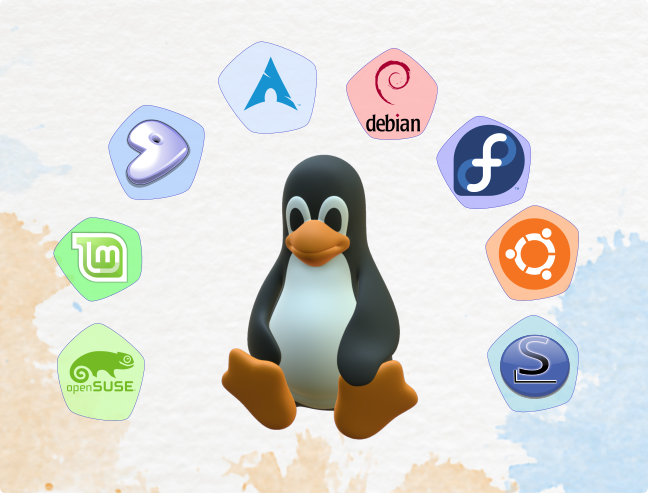
\includegraphics[height=3cm]{Linux_distro_logos_and_Tux.png}
	\end{column}
\end{columns}

	\begin{block}{Různorodost}
		\begin{itemize}
			\item Různé distribuce nabízejí odlišné možnosti a filosofie.
			\item  jednoduchost vs možnost si všechno nastavit po svém
			\item Fedora -- vybrána na základě zkušeností autorů kurzu.
		\end{itemize}
	\end{block}
\end{frame}



% Slide 4: Historie Linuxu
\begin{frame}{Historie Linuxu}
	\begin{block}{Vznik Linuxu}
		\begin{itemize}
			\item Linus Torvalds (finský student) vydal první verzi jádra Linuxu v roce 1991 jako hobby projekt.
			\item Před vydáním zaslal email komunitě, který začínal: \\
			I'm doing a (free) operating system (just a hobby, won't be big and professional like gnu) ...
			\item Torvalds navrhoval jméno „Freax“ jako free (svobodný) + freak (blázen) + x (unixový systém)
			\item správce FTP serveru jej pojmenoval Linux


		\end{itemize}
	\end{block}
\end{frame}

% Slide 5: Historie Linuxu
\begin{frame}{Historie Linuxu}
	\begin{block}{Vývoj a Růst Linuxu}
		\begin{itemize}
   			\item Linux získává popularitu díky otevřené povaze, stabilitě a flexibilitě.
   			\item Z 10 000 řádků kódu je projekt, který má přes 30 milionu řádků.
	        \item Serverová sféra: webové servery, databázové systémy, cloudové infrastruktury.
			\item Vestavěné systémy: spotřební elektronika, průmyslová zařízení, IoT.
			\item Mobilní prostředí: systémy jako Android.
			\item Superpočítače: mnoho z nejvýkonnějších superpočítačů běží na Linuxu.
		\end{itemize}
	\end{block}
\end{frame}

% Slide 6: Závěr
\begin{frame}{Závěr}
	\begin{block}{Co Nás Čeká}
		\begin{itemize}
			\item První krok – základy ovládání grafického prostředí GNOME.
		\end{itemize}
	\end{block}
\end{frame}

\end{document}
